\documentclass[12pt]{article}
\usepackage{amssymb}
\usepackage[UTF8]{ctex}
\usepackage{geometry}
\usepackage{units}
\usepackage{pifont}
\geometry{
	a4paper,
	total={150mm,237mm},
	left=30mm,
	top=27mm,
	}
\usepackage{amsmath}
\usepackage{enumerate}
\usepackage{lipsum}
\usepackage{graphicx}
\usepackage{hyperref}
\usepackage{indentfirst}
\usepackage[graphicx]{realboxes}
\usepackage{booktabs}
\usepackage{cases}
\usepackage{subfig}  
\usepackage{float}
\usepackage{xcolor}


\setlength{\parindent}{2em}
\title{Lab1}
\author{姓名:陈锐林,学号:21307130148}
\date{\today}

\begin{document}
\maketitle
\begin{Large}
    \noindent 实验一、内存分配实验\\
\end{Large}
\begin{large}
    \noindent 一、举例说明:\\
\end{large}
\hspace*{2em}根据题意,如果没有锁可能会导致较严重的后果。例如,如果两个进程同时对同一资源进行修改,又没有锁保护,会导致数据不一致。\\

\begin{large}
    \noindent 二、锁竞争:\\
\end{large}
\hspace*{2em}未修改前,kalloc只维护单个空闲链表,只有一个全局锁保护;虽然比较安全,但是也很可能出现锁竞争。同样地,如果多个线程同时分配一块内存,虽有锁的保护,但是会导致这些进程排队等候,导致性能下降。并且还可能导致死锁的问题出现;并且即使不涉及对同一内存访问,锁粒度太大也要很久等待。\\

\begin{large}
    \noindent 三、push\_off() and pop\_off:\\
\end{large}
\hspace*{2em}通过查看xv6的代码,以及查阅相关资料;得知这俩个函数的作用在于保证锁正常进行。push\_off函数用于禁用中断,保存CPU的中断状态,防止锁的获取被中断打断;pop\_off用于锁释放后,恢复之前保存的中断状态,允许重新中断。\\

\begin{large}
    \noindent 四、实验:\\
\end{large}
\noindent 1.实验思路:\\
\hspace*{2em}通过题目的hint,可从kmem出发;并且利用变量NCPU和cpuid()函数。首先,要为每个CPU分配一个列表,所以要将kmem改成数组形式,而大小即为NCPU;其次,在kinit()中要依次初始化;然后先解决简单的kfree(),这里只要使用cpuid()函数得到将要free的cpu即可,其他和之前一样。最后看kalloc()函数,这里分配内存时,首先考虑当前cpu(cpuid得到)的freelist是否有空间,有就直接插入;如果没有空间时,
就要考察能不能利用其他cpu下的空间,遍历其余cpu,如果某个页表还有空间就挪一半出来。
\newpage
\noindent 2.代码设计:\\
(1)对kmem/kinit()/kfree的修改:
\begin{figure*}[!h]
    \centering
    \subfloat[kmem]{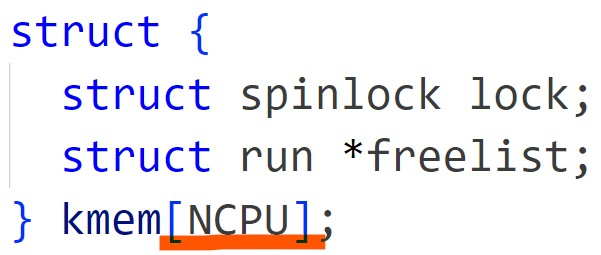
\includegraphics[width=4cm,height=2cm]{lab1-1.jpg} \label{X}}
    \hfill
    \subfloat[kinit]{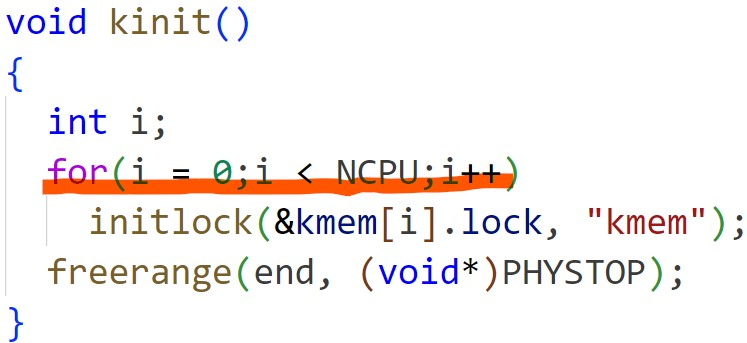
\includegraphics[width=4cm,height=3.3cm]{lab1-2.jpg} \label{Y}}
    \hfill
    \subfloat[kfree]{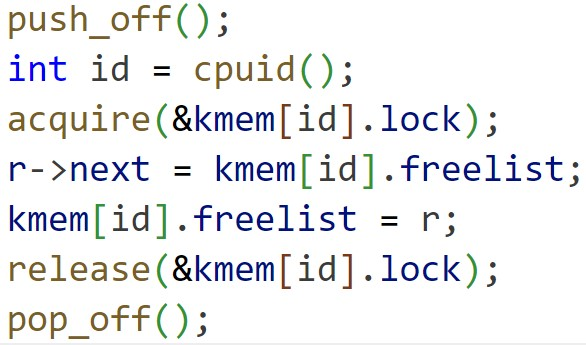
\includegraphics[width=4cm,height=4cm]{lab1-3.jpg} \label{Y}}
\end{figure*}

\noindent (2)对kalloc的修改:这里需要说明的是p1/p2/p3,其余就是正常的锁/开锁以及一些逻辑判断,基于有没有找到对应的内存。p1是原始指针,p3用来存储p1的值;而p2一次跑两格,意思是只取一半的空闲页表。
\begin{figure*}[!h]
    \centering
    \subfloat[part1]{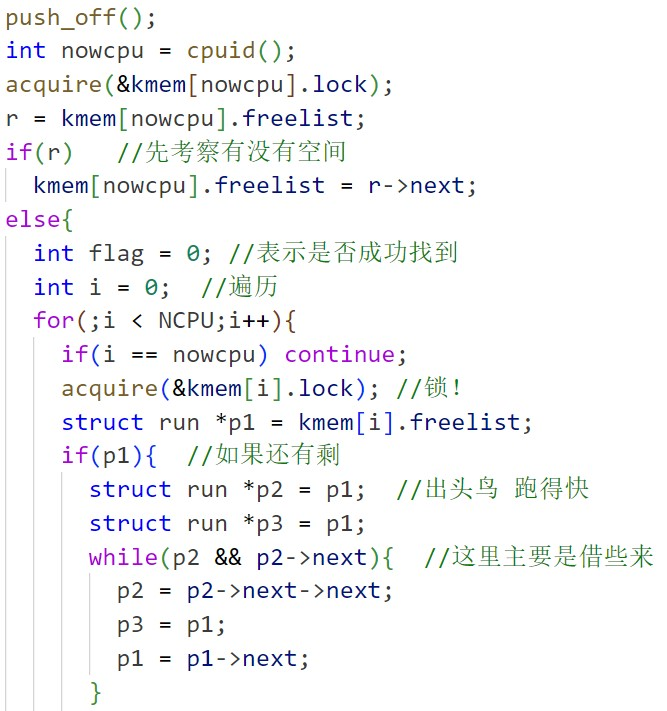
\includegraphics[width=7cm,height=9cm]{lab1-4.jpg} \label{X}}
    \hfill
    \subfloat[part2]{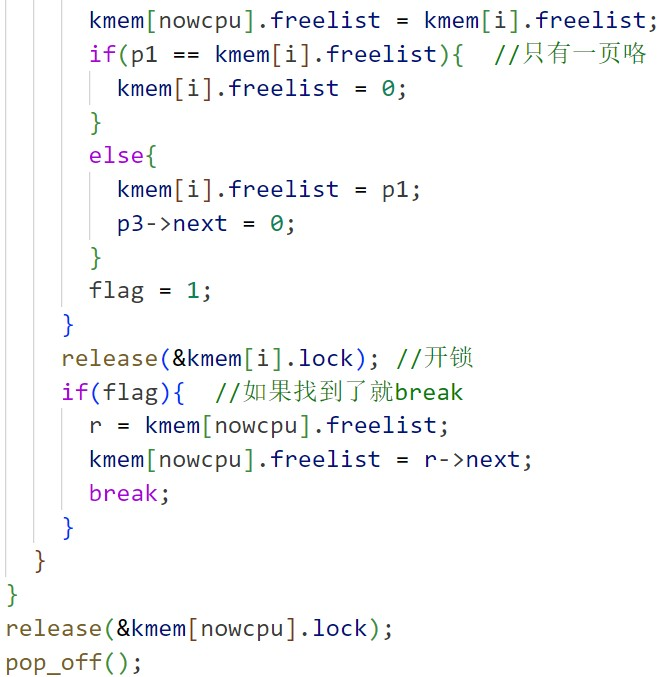
\includegraphics[width=7cm,height=9cm]{lab1-5.jpg} \label{Y}}
\end{figure*}\\
\newpage
\noindent 3.测试结果:
\begin{figure}[htbp]
    \begin{center}
        \includegraphics*[width=6cm,height=4cm]{lab1-6.jpg}
    \end{center}
\end{figure}\\

\begin{Large}
    \noindent 实验二:同步互斥实验\\
\end{Large}
\begin{large}
    \noindent 1.复旦早餐店:\\
\end{large}
(1)请写出题目中的互斥与同步关系:\par
同步1:鸡蛋灌饼进程和煎饼果子进程同时负责制作和售卖各自的早餐。\par
同步2:顾客队伍1和顾客队伍2分别同步排队,确保了顾客按照自己的需求购买早餐。\par
互斥1:老板和老板娘把做好的吃的放进篮子里这两件事是互斥的。\par
互斥2:两个顾客队列中只有一个能买到吃的,这是互斥的。\\
(2)伪代码:初始情况是篮子里已有一个吃的,以及假设是两列队伍都很长,所以老板和老板娘交替放鸡蛋灌饼和煎饼果子。并且顾客很多,不考虑顾客队列的人数变化(假设无穷无尽)\\
Process 1 \#(鸡蛋灌饼):\\
\hspace*{2em}while(true):\\
\hspace*{2em}wait(3):\\
\hspace*{4em}if 篮子为空:\\
\hspace*{6em}make鸡蛋灌饼,放入篮子\\
\hspace*{6em}call(2)\\

\noindent Process 2 \#(煎饼果子):\\
\hspace*{2em}while(true):\\
\hspace*{4em}wait(4)\\
\hspace*{4em}if 篮子为空:\\
\hspace*{6em}make煎饼果子,放入篮子\\
\hspace*{6em}call(1)
\newpage
\noindent Process 3 \#(买鸡蛋灌饼):\\
\hspace*{2em}while(true):\\
\hspace*{4em}wait(1)\\
\hspace*{4em}if 篮子有鸡蛋灌饼:\\
\hspace*{6em}买走\\

\noindent Process 4 \#(买煎饼果子):\\
\hspace*{2em}while(true):\\
\hspace*{4em}wait(2)\\
\hspace*{4em}if 篮子有煎饼果子:\\
\hspace*{6em}买走\\

\begin{large}
    \noindent 2.哲学家就餐问题:\\
\end{large}
\noindent (1)实现思路:\par
这个题目要求完成的部分其实不多,只要完成philosopher函数的部分即可。首先我们要定义当前索引为i的哲学家要拿起的筷子;其左手边为i号筷子,右手边为(i\%NUMBER\_OF\_PHILOSOPHERS)。第一部分是pickUp()函数,主要实现拿起筷子这一环节。可以直接调用pthread库中的函数,
对于i号哲学家,先试着拿起左筷子(即锁住左筷子);接着他进一步尝试锁住右筷子,如果返回错误,说明筷子正被人占用,那么他要主动放手(左右都要);过段时间后继续试着拿起左筷子,再右筷子。长此往复,直到吃完一波了才进入到第二部分。第二部分为putDown函数,即吃完了主动放下筷子,解开锁,
然后等待会进入下一阶段。\\
(2)代码实现:(主要是philosopher函数)
\begin{figure}[h]
    \centering
    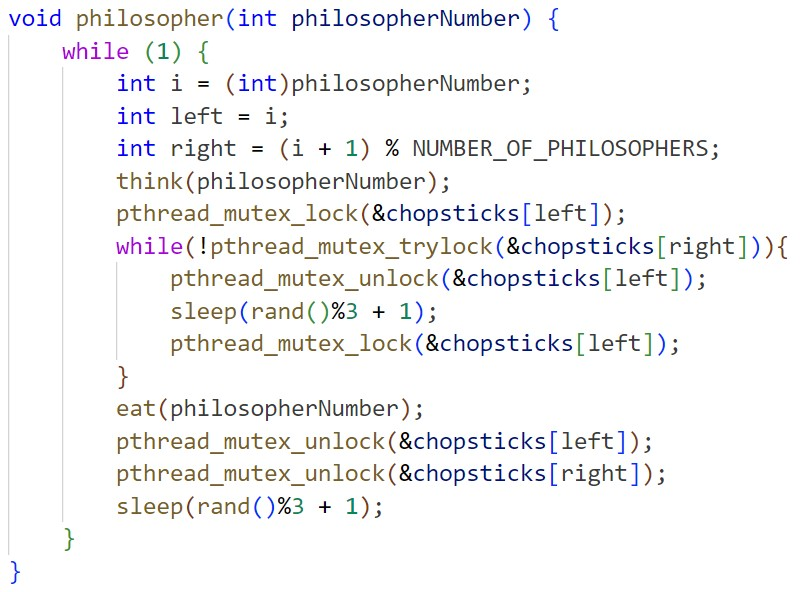
\includegraphics[width=9cm,height=8cm]{lab1-7.jpg}
\end{figure}\\
(3)测试结果:
\begin{figure}[h]
    \centering
    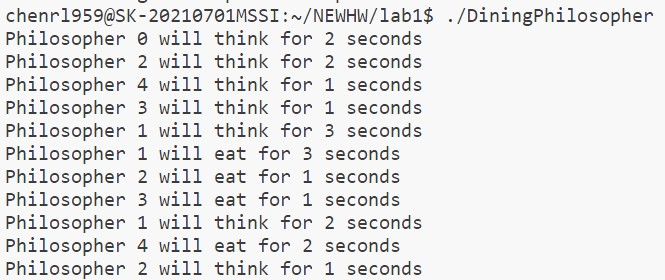
\includegraphics[width=10cm,height=6cm]{lab1-8.jpg}
\end{figure}\\
\end{document} 